% ----------------------------------------------------
\begin{frame}
  \titlepage
\end{frame}
% ----------------------------------------------------
\note{Tema central de la sesión: si la guerra es tan costosa para todos, por qué ocurre? Vamos a ver que los intereses en conflicto son condición necesaria pero no suficiente. Lo que explica la guerra es el fracaso de la negociación, y hay tres grandes razónes por las que falla: información incompleta, problemas de compromiso y bienes indivisibles.}

% ----------------------------------------------------
\begin{frame}[plain]
  \begin{tikzpicture}[remember picture, overlay]
    \node[at = (current page.center), yshift = 0cm] (cover) {%
      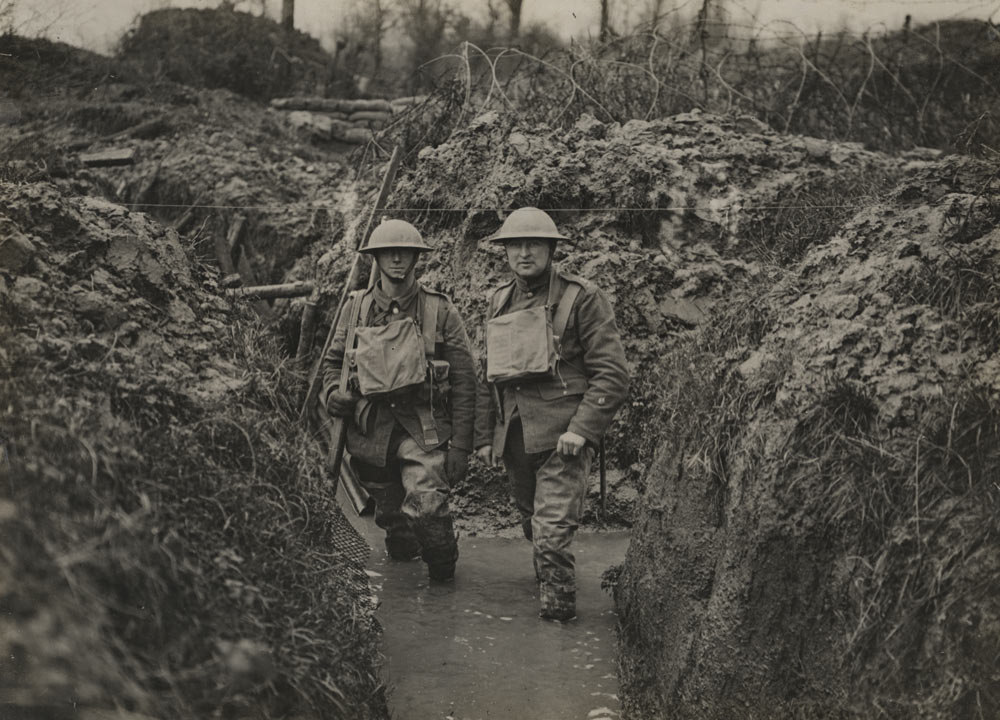
\includegraphics[keepaspectratio, height=\paperheight]{../img/wwi_trenches}};
  \end{tikzpicture}
\end{frame}
% ----------------------------------------------------
\note{Trincheras de la Primera Guerra Mundial. Mas de 15 millones de muertos en cuatro años. Los líderes europeos creían que la guerra terminaría antes de Navidad de 1914. Si era tan catastrófica, por qué no la evitaron? Esta imagen debe provocar la pregunta que guia toda la sesión.}

% ----------------------------------------------------
\begin{frame}
\frametitle{El puzzle de la guerra}
\centering

\begin{itemize}
  \item La guerra es \textbf{enormemente costosa}
  \begin{itemize}
    \item Vidas humanas, destrucción material, costes económicos
  \end{itemize}
  \item<2-> Si todos pierden con la guerra, \textit{por qué no negocian?}
  \vspace{8pt}
  \item<3-> La mayoría de los conflictos \textbf{si} se resuelven sin guerra
  \item<3-> La guerra es la \textbf{excepción}, no la regla
  \vspace{8pt}
  \item<4-> No basta con saber \textit{por qué luchan}, sino \textit{por qué falla la negociación}
\end{itemize}

\end{frame}
% ----------------------------------------------------
\note{Plantear el puzzle con claridad. No basta con decir que tenían intereses enfrentados. Dato: en cualquier año dado, el porcentaje de Estados en guerra es muy bajo. Hay miles de disputas que se resuelven sin violencia. La paz no se explica por falta de desacuerdos -- los hay todo el tiempo. Lo que necesitamos explicar es por qué a veces falla la negociación. Esta es la intuición central de Fearon (1995), que transforma como los politólogos estudian la guerra.}


% ====================================================
\section{Intereses en conflicto}
% ====================================================

% ----------------------------------------------------
\begin{frame}
\frametitle{¿Por qué luchan los Estados?}
\centering

\begin{itemize}
  \item \textbf{Territorio}
  \begin{itemize}
    \item Recursos naturales, posición estratégica, identidad étnica o cultural
    \item Causa históricamente más frecuente de guerra
  \end{itemize}
  \item<2-> \textbf{Políticas de otro Estado}
  \begin{itemize}
    \item Armas de destrucción masiva, violaciones de derechos humanos
  \end{itemize}
  \item<3-> \textbf{Régimen político}
  \begin{itemize}
    \item Composición del gobierno de otro país
    \item Cambio de régimen, intervenciones
  \end{itemize}
\end{itemize}

\end{frame}
% ----------------------------------------------------
\note{Tres grandes categorías de conflictos de interés según FLS. Territorio: Iran-Irak (petróleo y acceso al Shatt al-Arab), Israel-Siria (Altos del Golan), India-Pakistan (Cachemira). Mas de la mitad de las guerras interestatales en los últimos 300 años fueron por territorio. Políticas: la invasión de Irak en 2003 se justificó por las armas de destrucción masiva; las sanciones contra Corea del Norte buscan frenar su programa nuclear. Régimen: toda la Guerra Fría esta llena de ejemplos de intervenciones para cambiar gobiernos -- Vietnam, Guatemala, Chile. Pero es fundamental que los estudiantes entiendan que los intereses en conflicto son condición necesaria pero no suficiente para la guerra.}

% ----------------------------------------------------
\begin{frame}
\frametitle{Los intereses no son suficientes}
\centering

\begin{itemize}
  \item Los intereses en conflicto son \textbf{constantes}
  \begin{itemize}
    \item Siempre hay disputas territoriales, políticas, etc.
  \end{itemize}
  \item<2-> Pero las guerras son \textbf{raras}
  \item<2-> Hay algo más que convierte un conflicto de intereses en guerra
  \vspace{8pt}
  \item<3-> Necesitamos entender por qué falla la \textbf{negociación}
\end{itemize}

\end{frame}
% ----------------------------------------------------
\note{Slide de transición clave. Si los intereses en conflicto bastasen para explicar la guerra, habría guerras constantemente. España y Reino Unido tienen una disputa territorial por Gibraltar desde hace 300 años -- y nunca han ido a la guerra por ello. Argentina y Chile resolvieron sus disputas fronterizas mediante arbitraje. Lo que convierte un conflicto de intereses en guerra no es la intensidad de los intereses, sino el fracaso de la negociación. Esto nos lleva al modelo de negociación.}

% ----------------------------------------------------
\begin{frame}[plain]
  \begin{tikzpicture}[remember picture, overlay]
    \node[at = (current page.center), yshift = 0cm] (cover) {%
      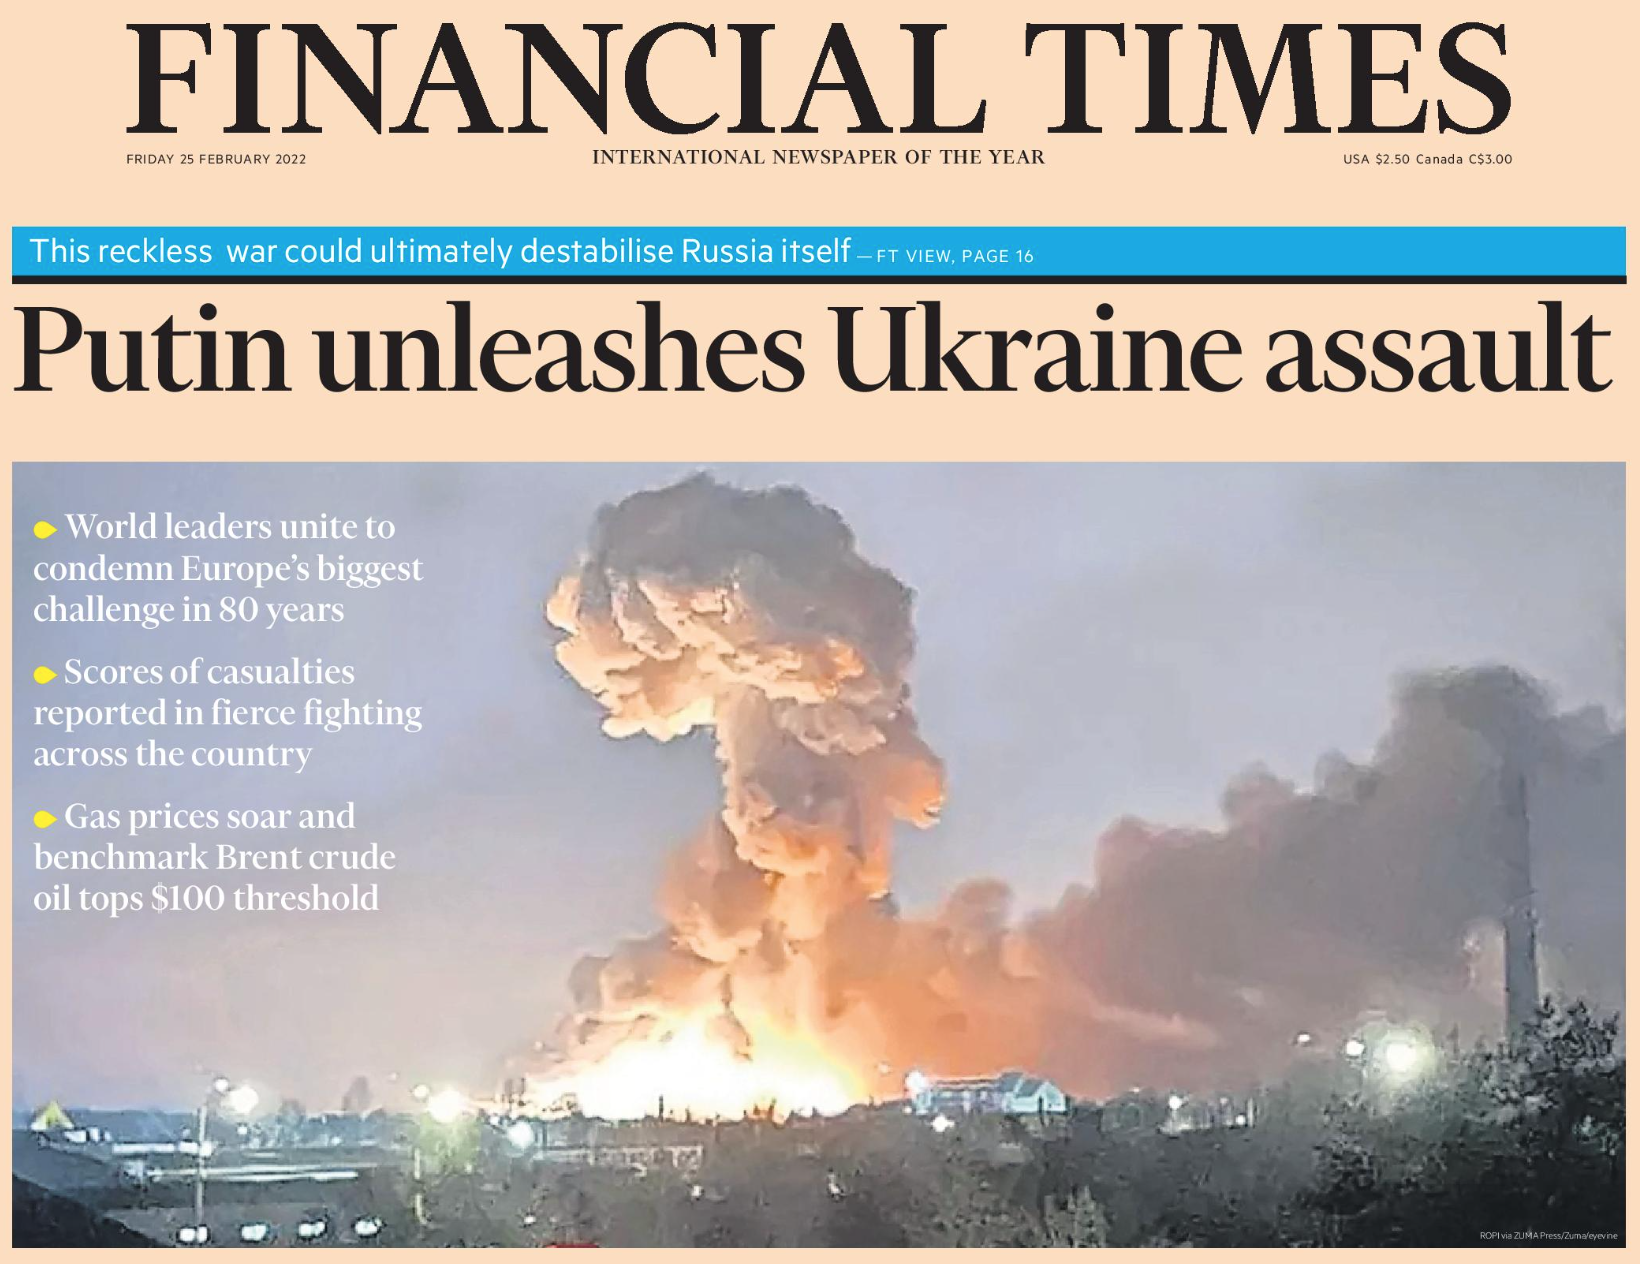
\includegraphics[keepaspectratio, height=\paperheight]{../img/ukraine_war}};
  \end{tikzpicture}
\end{frame}
% ----------------------------------------------------
\note{Guerra de Ucrania. Un conflicto que en 2022 sorprendió a muchos analistas, pese a que habia señales claras. Rusia y Ucrania tenían una disputa sobre territorio (Crimea, Donbas), políticas (expansion de la OTAN) y régimen (Rusia quería un gobierno afin en Kiev). Pero la pregunta sigue siendo: por qué no llegaron a un acuerdo? Los costes de la guerra han sido enormes para todos.}


% ====================================================
\section{El modelo de negociación}
% ====================================================

% ----------------------------------------------------
\begin{frame}
\frametitle{Negociación bajo amenaza de fuerza}
\centering

\begin{itemize}
  \item No hay tribunales ni policía a nivel internacional
  \item Los Estados resuelven sus conflictos mediante \textbf{negociación}
  \item<2-> \textbf{Crisis:} al menos un Estado amenaza con usar la fuerza
  \begin{itemize}
    \item ``Acepta mis demandas, o si no...''
  \end{itemize}
  \item<2-> \textit{Crisis bargaining} / diplomacia coercitiva
\end{itemize}

\end{frame}
% ----------------------------------------------------
\note{En la política doméstica, si alguien te roba puedes acudir a los tribunales y la policía hará cumplir la sentencia. En el sistema internacional no existe ese mecanismo. No hay un gobierno mundial. Los conflictos se resuelven entre las propias partes, y la amenaza de fuerza es una herramienta de negociación. Ejemplos: el ultimatum de Bush a Saddam Hussein (48 horas para irse de Irak, 2003); la concentración de tropas rusas en la frontera ucraniana en 2021-22; el bloqueo naval de Kennedy durante la crisis de los misiles. La negociación coercitiva combina amenazas con ofertas.}

% ----------------------------------------------------
\begin{frame}
\frametitle{El rango de negociación}
\centering

\vspace{-5pt}
\begin{tikzpicture}[scale=0.85]
  % The bar representing the disputed good
  \fill[accent!15] (0, 0) rectangle (10, 0.6);
  \draw[thick] (0, 0) rectangle (10, 0.6);

  % Labels for ideal points
  \node[font=\footnotesize, anchor=south] at (0, 0.7) {Ideal A};
  \node[font=\footnotesize, anchor=south] at (10, 0.7) {Ideal B};

  % War outcome (expected)
  \draw[thick, accent2, dashed] (5.5, -0.2) -- (5.5, 0.8);
  \node[font=\scriptsize, accent2, anchor=south] at (5.5, 0.85) {Resultado esperado};

  % Bargaining range
  \draw[thick, accent, <->] (3.8, -0.5) -- (7.2, -0.5);
  \node[font=\scriptsize, accent, anchor=north] at (5.5, -0.55) {\textbf{Rango de negociación}};

  % Value of war for each side
  \draw[thick, accent!60] (3.8, -0.2) -- (3.8, 0.8);
  \node[font=\tiny, anchor=south east] at (3.7, 0.85) {Valor guerra A};
  \draw[thick, accent!60] (7.2, -0.2) -- (7.2, 0.8);
  \node[font=\tiny, anchor=south west] at (7.3, 0.85) {Valor guerra B};

  % Cost arrows
  \draw[thick, red!60, <->] (3.8, -1.1) -- (5.5, -1.1);
  \node[font=\tiny, red!60!black] at (4.65, -1.4) {Costes de A};
  \draw[thick, red!60, <->] (5.5, -1.1) -- (7.2, -1.1);
  \node[font=\tiny, red!60!black] at (6.35, -1.4) {Costes de B};

\end{tikzpicture}

\vspace{8pt}
\begin{itemize}
  \item[\color{accent}$\bullet$] \footnotesize Los costes de guerra crean un \textbf{rango de acuerdos} que ambos prefieren a luchar
\end{itemize}

\end{frame}
% ----------------------------------------------------
\note{Diagrama central del tema. La barra horizontal representa el bien en disputa (por ejemplo, un territorio). A quiere todo para si (extremo izquierdo); B quiere todo para si (extremo derecho). Si van a la guerra, el resultado esperado está en algun punto de la barra, pero ambos pagan costes (vidas, dinero, destrucción). Esos costes ``encogen'' lo que cada lado obtiene de la guerra, creando una zona de acuerdos que ambos prefieren a pelear. Cuanto mayores son los costes de guerra, más amplio es el rango de negociación. Implicacion fundamental: siempre que la guerra tenga costes para ambos bandos, existe un rango de negociación. Siempre hay acuerdos que ambos prefieren a la guerra.}

% ----------------------------------------------------
\begin{frame}
\frametitle{Ejemplo numérico}
\centering

\footnotesize
\begin{itemize}
  \item A y B disputan un territorio valorado en \textbf{100 millones}
  \item A espera ganar la guerra; costes de A = 30M
  \vspace{8pt}
  \item<2-> Valor de guerra para A = 100 $-$ 30 = \textbf{70M}
  \item<2-> A acepta cualquier acuerdo que le de $\geq$ 70M
  \vspace{8pt}
  \item<3-> B espera perder; costes de B = 20M
  \item<3-> Valor de guerra para B = 0 $-$ 20 = \textbf{$-$20M}
  \item<3-> B acepta cualquier acuerdo que le cueste $\leq$ 20M
  \vspace{8pt}
  \item<4-> \textbf{Rango:} A recibe entre 70 y 80M $\rightarrow$ ambos prefieren negociar
\end{itemize}

\end{frame}
% ----------------------------------------------------
\note{Ejemplo numérico para fijar la intuición. El territorio vale 100M. A espera ganar, pero la guerra le cuesta 30M, así que su valor neto es 70M. A acepta cualquier acuerdo que le de al menos 70M. Para B: espera perder el territorio (valor 0) y además pagar 20M en costes. Cualquier acuerdo donde B pierda menos de 20M es mejor que luchar. Esto significa que A puede recibir entre 70M (lo minimo que acepta) y 80M (lo maximo que B está dispuesto a ceder, ya que ceder 80M a A equivale a perder 80M, que es mejor que perder 100M + 20M de costes). Cualquier reparto en ese rango es mutuamente preferible a la guerra. Pregunta clave: si este rango siempre existe, por qué hay guerras?}

% ----------------------------------------------------
\begin{frame}
\centering
\vspace{30pt}

{\large ¿Se os ocurre un conflicto real en el que ambos bandos habrían estado mejor con un acuerdo negociado?}

\vspace{15pt}
\footnotesize ¿Por qué no lo alcanzaron?

\end{frame}
% ----------------------------------------------------
\note{Pregunta de discusión para activar la participación. Respuestas posibles: la Primera Guerra Mundial (todos perdieron -- cuatro imperios colapsaron, 15 millones de muertos), la guerra de Iran-Irak (8 años, más de un millón de muertos, ningún cambio territorial significativo), la guerra de Irak 2003 (EE.UU. habría evitado una ocupación costosísima). Usar las respuestas para conectar con las tres causas de fracaso que vamos a ver a continuación. Insistir en que la pregunta no es solo por qué luchan, sino por qué no alcanzan el acuerdo que ambos preferirían.}


% ====================================================
\section{Compelencia y disuasión}
% ====================================================

% ----------------------------------------------------
\begin{frame}
\frametitle{Compelencia y disuasión}
\centering

\begin{itemize}
  \item \textbf{Compelencia} (\textit{compellence}):
  \begin{itemize}
    \item Amenazar con la fuerza para \textit{cambiar} el statu quo
    \item ``Dame \textit{x}, o si no...''
  \end{itemize}
  \vspace{8pt}
  \item<2-> \textbf{Disuasion} (\textit{deterrence}):
  \begin{itemize}
    \item Amenazar con la fuerza para \textit{preservar} el statu quo
    \item ``No hagas \textit{x}, o si no...''
  \end{itemize}
  \vspace{8pt}
  \item<3-> Disuasion \textbf{general} vs. \textbf{extendida}
  \begin{itemize}
    \item General: ``no me ataques''
    \item Extendida: ``no ataques a mi aliado'' (más difícil)
  \end{itemize}
\end{itemize}

\end{frame}
% ----------------------------------------------------
\note{Dos tipos fundamentales de amenazas. Compelencia: EE.UU. exige a los talibanes que entreguen a Bin Laden en 2001; Irak exige a Kuwait que ceda territorio y condone deuda en 1990; Rusia exige a Ucrania que se comprometa a no entrar en la OTAN. Disuasion general: todos los Estados la practican (si me atacas, me defiendo). Disuasion extendida: EE.UU. protege a Corea del Sur (50.000 soldados desplegados), la OTAN protege a los países bálticos. La disuasión extendida es más difícil porque el disuador no esta directamente amenazado. Pregunta clásica de la Guerra Fría: sacrificaría EE.UU. Nueva York para defender Hamburgo o Paris?}

% ----------------------------------------------------
\begin{frame}
\frametitle{La disuasión nuclear}
\centering

\begin{itemize}
  \item La disuasión funciona mejor cuando los costes de la guerra son \textbf{enormes}
  \item<2-> Armas nucleares: \textbf{destrucción mutua asegurada} (MAD)
  \begin{itemize}
    \item Un ataque nuclear garantiza una represalia devastadora
    \item Nadie puede ``ganar'' una guerra nuclear
  \end{itemize}
  \vspace{8pt}
  \item<3-> Las armas nucleares han hecho que las guerras entre grandes potencias sean \textbf{demasiado costosas}
  \item<3-> No ha habido guerra directa entre potencias nucleares
\end{itemize}

\end{frame}
% ----------------------------------------------------
\note{La disuasión nuclear es el ejemplo más extremo del rango de negociación: los costes son tan astronómicos que el rango de acuerdos preferibles a la guerra es inmenso. Desde 1945, no ha habido guerra directa entre grandes potencias. Antes de las armas nucleares, las grandes potencias luchaban entre si regularmente (las dos guerras mundiales son el caso más extremo). Pero la disuasión nuclear tiene sus propios problemas: la crisis de los misiles de Cuba en 1962 mostró lo cerca que se puede llegar del desastre. Además, la disuasión nuclear no impide las guerras convencionales (Vietnam, Corea, Irak) ni las guerras proxy.}


% ====================================================
\section{Información incompleta}
% ====================================================

% ----------------------------------------------------
\begin{frame}
\frametitle{¿Por qué falla la negociación? (I)}
\centering

{\Large \textbf{Información incompleta}}

\vspace{15pt}

\begin{itemize}
  \item Los Estados no conocen con certeza las \textbf{capacidades} ni la \textbf{determinación} del adversario
  \item<2-> \textbf{Capacidades:} tropas, armamento, tecnología, aliados
  \item<2-> \textbf{Determinación} (\textit{resolve}): disposición a asumir costes
  \vspace{8pt}
  \item<3-> Si no se dónde está el rango de negociación, puedo hacer demandas que el otro rechaza
\end{itemize}

\end{frame}
% ----------------------------------------------------
\note{Primera causa de fracaso en la negociación. Analogía del poker: conoces tus cartas pero no las del adversario. Las capacidades son parcialmente observables (satelites, informes de inteligencia) pero no del todo. La determinación es aun más difícil de medir: cuantas vidas está dispuesto a sacrificar un país por un territorio? Depende de factores políticos, ideológicos, psicológicos. Ejemplo: Saddam Hussein creía que EE.UU. no aceptaria 10.000 muertos en una batalla. Se equivocaba. China advirtio a EE.UU. en 1950 de que intervendría si cruzaban el paralelo 38 en Corea. Dean Acheson lo descartó como un farol. Resultado: 600.000 soldados chinos entraron en la guerra.}

% ----------------------------------------------------
\begin{frame}
\frametitle{El dilema riesgo-beneficio}
\centering

\begin{itemize}
  \item Cuando hay incertidumbre, cada Estado enfrenta un dilema:
  \vspace{8pt}
  \item<2-> \textbf{Ceder mucho} $\rightarrow$ paz segura, pero mal acuerdo
  \item<2-> \textbf{No ceder} $\rightarrow$ mejor acuerdo si funciona, pero riesgo de guerra
  \vspace{8pt}
  \item<3-> Este \textbf{trade-off} puede llevar racionalmente a la guerra
  \item<3-> La guerra no requiere líderes irracionales o locos
\end{itemize}

\end{frame}
% ----------------------------------------------------
\note{El trade-off riesgo-beneficio es crucial para entender que la guerra puede ser resultado de decisiones racionales. Kuwait en 1990: podría haber cedido a todas las demandas de Irak y evitado la invasión. Pero no quería paz a cualquier precio. Eligió no ceder, apostando a que Saddam estaba faroleando. No fue irracional: era una apuesta razonable dada la incertidumbre sobre las intenciones de Saddam. Lo mismo para Ucrania en 2022: podría haber aceptado las demandas de Putin, pero eso habría significado ceder soberanía. La guerra puede ocurrir aunque ambos bandos sean racionales, simplemente porque no tienen suficiente información sobre el otro.}

% ----------------------------------------------------
\begin{frame}
\frametitle{El problema de la credibilidad}
\centering

\begin{itemize}
  \item ¿Por qué no se comunican la información?
  \item<2-> Los Estados tienen incentivos para \textbf{mentir o exagerar}
  \begin{itemize}
    \item Ocultar debilidades (parecer más fuerte)
    \item Farolear (\textit{bluff}): amenazar sin intención de cumplir
    \item Exagerar la determinación para obtener un mejor acuerdo
  \end{itemize}
  \vspace{8pt}
  \item<3-> Un mensaje solo es útil si es \textbf{creíble}
  \item<3-> El adversario siempre se pregunta: \textit{me esta diciendo la verdad?}
\end{itemize}

\end{frame}
% ----------------------------------------------------
\note{Problema central de la comunicación estratégica. Si un Estado dice que está dispuesto a luchar, el adversario no sabe si es verdad o es un farol. Ejemplo: Hitler envió tropas a Renania en 1936 (zona desmilitarizada por el Tratado de Versalles). Francia y Gran Bretana no reaccionaron. Hay evidencia de que era un farol: las tropas tenían ordenes de retirarse si Francia intervenía. Si Francia hubiera llamado al farol, la historia podría haber sido muy diferente. Otro ejemplo: China y Corea en 1950 -- el mensaje de que China intervendría fue descartado como bluff, pero era verdad. El dilema es como separar las señales sinceras de los faroles.}


% ====================================================
\section{Señales costosas}
% ====================================================

% ----------------------------------------------------
\begin{frame}
\frametitle{¿Cómo hacer creíbles las amenazas?}
\centering

\begin{itemize}
  \item Para que una amenaza sea creíble, debe ser \textbf{costosa} de hacer
  \begin{itemize}
    \item Algo que no harías si estuvieras faroleando
  \end{itemize}
  \vspace{8pt}
  \item<2-> Tres mecanismos:
  \begin{enumerate}
    \item<2-> \textbf{Brinksmanship} (diplomacia al borde del abismo)
    \item<3-> \textbf{Atarse las manos} (\textit{tying hands})
    \item<4-> \textbf{Pagar para tener poder} (\textit{paying for power})
  \end{enumerate}
\end{itemize}

\end{frame}
% ----------------------------------------------------
\note{Idea general de Thomás Schelling (Premio Nobel de Economia, 2005): las amenazas baratas no son creíbles porque cualquiera puede hacerlas. Para demostrar que hablas en serio, tienes que hacer algo que te cueste algo que no harías si fueras un farolero. Es la misma lógica que en la vida cotidiana: si alguien dice que te va a devolver un prestamo, le crees más si pone su casa como garantía. La señal es costosa, y por eso es creíble. Vamos a ver tres formas concretas de enviar señales costosas en las relaciones internacionales.}

% ----------------------------------------------------
\begin{frame}
\frametitle{Brinksmanship}
\centering

\begin{itemize}
  \item Aumentar deliberadamente el riesgo de guerra \textit{accidental}
  \item<2-> ``El borde del precipicio no es un acantilado donde uno se para y decide si salta; es una \textbf{pendiente resbaladiza}'' (Schelling)
  \vspace{8pt}
  \item<3-> Cada bando sube la apuesta hasta que uno cede...
  \item<3-> ...o caen juntos
  \vspace{8pt}
  \item<4-> Ejemplo clásico: \textbf{crisis de los misiles de Cuba (1962)}
\end{itemize}

\end{frame}
% ----------------------------------------------------
\note{El brinksmanship no es una amenaza de empezar una guerra deliberadamente -- eso no sería creíble si la guerra es catastrófica, especialmente una guerra nuclear. Es crear una situacion donde la guerra puede empezar por accidente o escalada incontrolada. Kennedy impuso un bloqueo naval a Cuba; Jrushchov tenía barcos soviéticos acercandose. Nadie quería una guerra nuclear, pero ambos tomaron medidas que aumentaban el riesgo de un incidente que desencadenase la escalada. Un incidente real: un U-2 americano fue derribado sobre Cuba. Un submarino soviético casí lanzó un torpedo nuclear. La disposición a asumir ese riesgo separa a los que van en serio de los que farolean.}

% ----------------------------------------------------
\begin{frame}[plain]
  \begin{tikzpicture}[remember picture, overlay]
    \node[at = (current page.center), yshift = 0cm] (cover) {%
      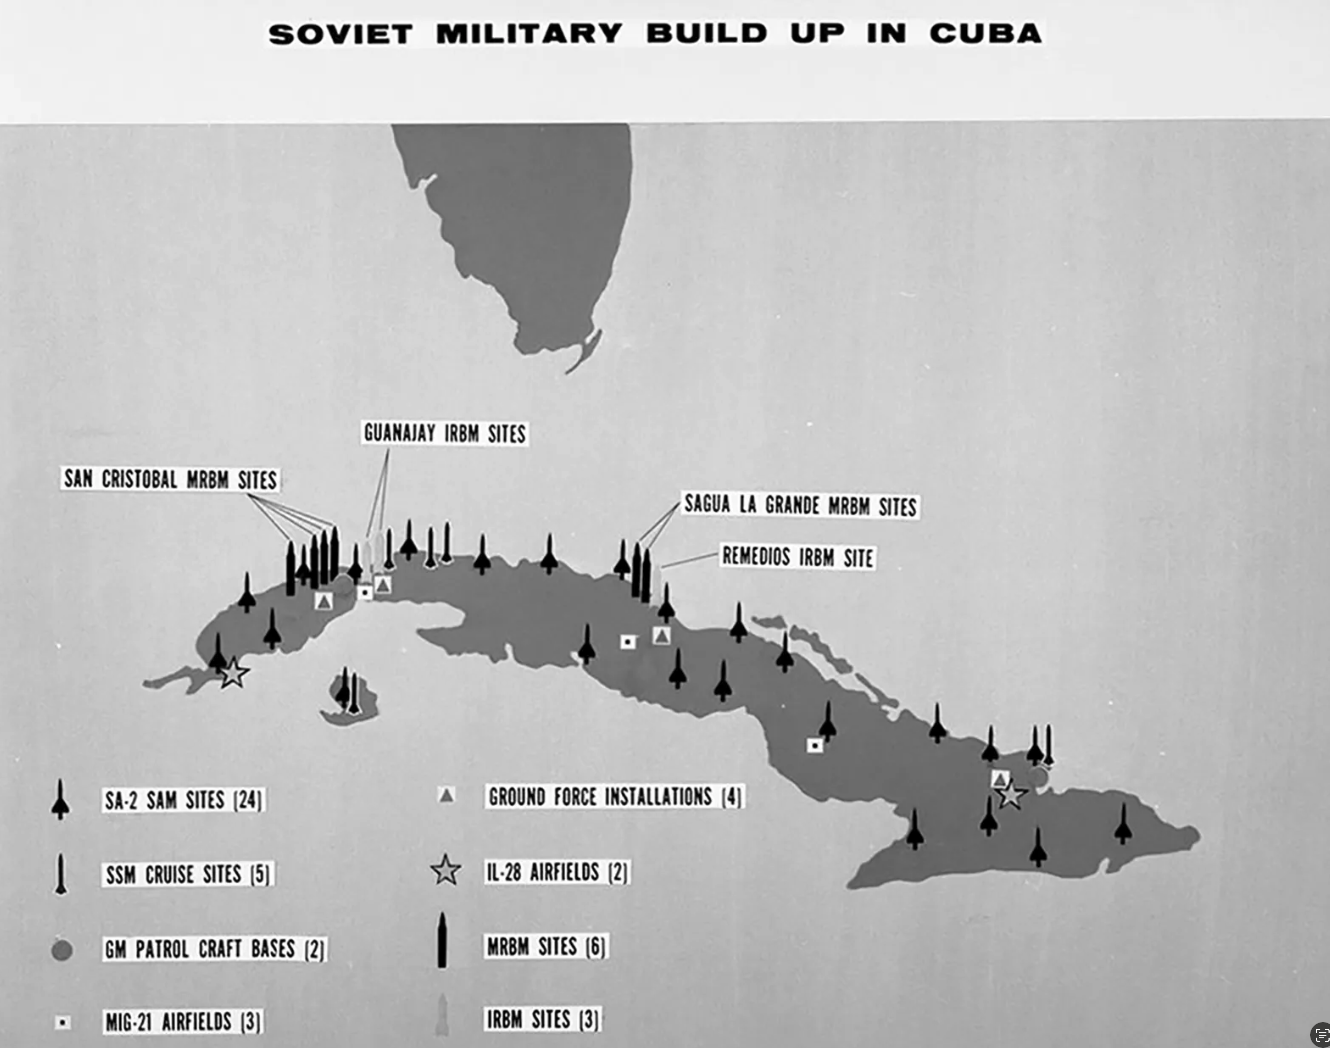
\includegraphics[keepaspectratio, height=\paperheight]{../img/cuban_missile_crisis}};
  \end{tikzpicture}
\end{frame}
% ----------------------------------------------------
\note{Crisis de los misiles de Cuba (octubre 1962). Fotografias aereas revelaron que la URSS estaba instalando misiles nucleares en Cuba, a 150 km de Florida. Kennedy impuso un bloqueo naval. Durante 13 dias, el mundo estuvo al borde de la guerra nuclear. Un submarino soviético (B-59) casí lanzó un torpedo nuclear al ser bombardeado con cargas de profundidad. Solo la negativa de un oficial, Vasili Arjipov, lo impidió. Al final, Jrushchov retiró los misiles a cambio de la promesa de EE.UU. de no invadir Cuba y la retirada secreta de misiles americanos de Turquia. Es el ejemplo perfecto de brinksmanship: ambos sabrían que la guerra sería catastrófica, pero la disposición a correr riesgos fue la señal.}

% ----------------------------------------------------
\begin{frame}
\frametitle{Atarse las manos (\textit{tying hands})}
\centering

\begin{itemize}
  \item Hacer declaraciones públicas o acciones de las que sea difícil echarse atrás
  \item<2-> Si el líder no cumple, paga \textbf{costes de audiencia}
  \begin{itemize}
    \item Reputación internacional dañada
    \item Castigo electoral doméstico
  \end{itemize}
  \vspace{8pt}
  \item<3-> Bush (1990): ``This will not stand'' $\rightarrow$ credibilidad alta
  \item<3-> Obama (2012): ``línea roja'' en Siria $\rightarrow$ no actuó $\rightarrow$ credibilidad dañada
\end{itemize}

\end{frame}
% ----------------------------------------------------
\note{Costes de audiencia (audience costs). Cuando un líder hace una declaración publica, se juega su reputación. Bush tras la invasión de Kuwait: desplegó 500.000 tropas y declaró publicamente que la invasión no sería aceptada. Retroceder habría sido políticamente devastador, así que la amenaza era altamente creíble. Contraste: Obama dijo en 2012 que el uso de armas químicas en Siria sería una línea roja. Cuando Assad las uso en agosto de 2013, Obama no ataco. Fue muy criticado por haber hecho una amenaza vacía. La lección: atarse las manos es poderoso pero peligroso. Si te atas las manos y el adversario no cede, estas obligado a luchar. Y si no cumples, tu credibilidad futura queda comprometida.}

% ----------------------------------------------------
\begin{frame}
\frametitle{Pagar para tener poder (\textit{paying for power})}
\centering

\begin{itemize}
  \item Tomar medidas costosas para aumentar las capacidades militares
  \begin{itemize}
    \item Movilización de tropas, aumentó del gasto militar
  \end{itemize}
  \vspace{8pt}
  \item<2-> Doble efecto:
  \begin{itemize}
    \item Reduce el coste de cumplir la amenaza (estas más preparado)
    \item Señala que el Estado se toma en serio la disputa
  \end{itemize}
  \vspace{8pt}
  \item<3-> Ejemplo: Kennedy aumentó el ejército en 350.000 soldados durante la crisis de Berlin (1961)
\end{itemize}

\end{frame}
% ----------------------------------------------------
\note{Tercer mecanismo de señalizacion costosa. Las movilizaciones militares no solo son preparativos para la guerra: también son señales. Si un Estado gasta grandes cantidades de dinero y recursos, demuestra que le importa lo suficiente como para luchar. Kennedy llamó a reservistas -- personas que ya habían terminado su servicio militar y tenían familias y trabajos civiles. Eso es políticamente costoso (genera protestas, afecta la economía), lo que hace la señal más creíble. Pero estas ``curas'' para la información incompleta son peligrosas en si mismas: el brinksmanship crea riesgo de accidente; atarse las manos puede impedir la flexibilidad diplomática; y las movilizaciones pueden provocar al adversario a atacar primero, como veremos con los problemas de compromiso.}


% ====================================================
\section{Problemas de compromiso}
% ====================================================

% ----------------------------------------------------
\begin{frame}
\frametitle{¿Por qué falla la negociación? (II)}
\centering

{\Large \textbf{Problemas de compromiso}}

\vspace{15pt}

\begin{itemize}
  \item A veces el acuerdo pacífico existe, pero...
  \item<2-> Puedo confiar en que el adversario \textbf{cumplirá} el acuerdo en el futuro?
  \item<3-> Si no hay forma de garantizarlo, puede ser mejor luchar \textit{ahora}
\end{itemize}

\end{frame}
% ----------------------------------------------------
\note{Segunda gran categoria de causas de la guerra. La diferencia con la información incompleta: aqui ambos Estados pueden conocer perfectamente las capacidades y la determinación del otro. El problema no es la falta de información sino la falta de confianza en que el acuerdo se respetara. En la política doméstica, los tribunales y la policía hacen cumplir los contratos. En la política internacional, no hay equivalente. El sistema internacional es anárquico -- no hay autoridad superior que obligue a cumplir los acuerdos. Tres variantes de este problema: bienes que dan poder, guerra preventiva y guerra preemptiva.}

% ----------------------------------------------------
\begin{frame}
\frametitle{Bienes que dan poder}
\centering

\begin{itemize}
  \item Cuando el bien en disputa es fuente de \textbf{poder futuro}
  \begin{itemize}
    \item Territorio estratégico, armas nucleares
  \end{itemize}
  \vspace{8pt}
  \item<2-> Ceder hoy $\rightarrow$ el adversario se fortalece $\rightarrow$ manana exige más
  \vspace{8pt}
  \item<3-> Ejemplo: \textbf{Libia (2003-2011)}
  \begin{itemize}
    \item<3-> Gadafi renunció a armas químicas y nucleares en 2003
    \item<3-> Prometieron no atacar... en 2011 fue intervenido y derrocado
  \end{itemize}
  \vspace{8pt}
  \item<4-> Lección para Corea del Norte: \textit{nunca} renunciar a las armas nucleares
\end{itemize}

\end{frame}
% ----------------------------------------------------
\note{El caso de Libia es muy instructivo. Gadafi renunció a su programa de armas de destrucción masiva en 2003 a cambio de normalización con EE.UU. y Reino Unido. Parecía un éxito diplomático. Pero en 2011, cuando estalló una rebelión, la OTAN intervino y Gadafi fue derrocado y asesinado. La lección que extrajeron otros régimenes fue clara: las promesas de no atacar no son duraderas. Corea del Norte cita explícitamente el caso de Libia como razón para no negociar su programa nuclear. Otro ejemplo: las islas Senkaku/Diaoyu entre China y Japón -- el control de las islas afecta al equilibrio militar regional en el Pacífico. Si ceder un bien te hace más vulnerable y no hay garantía de que el adversario no lo explotará, puede ser racional preferir la guerra.}

% ----------------------------------------------------
\begin{frame}
\frametitle{Guerra preventiva}
\centering

\begin{itemize}
  \item Cuando el equilibrio de poder está cambiando
  \begin{itemize}
    \item Crecimiento económico desigual, nuevas tecnologías
  \end{itemize}
  \vspace{8pt}
  \item<2-> El Estado que se debilita prefiere luchar \textbf{hoy} antes de ser más debil \textbf{manana}
  \item<2-> No puede confiar en que el Estado creciente no explotará su ventaja
  \vspace{8pt}
  \item<3-> Ejemplos:
  \begin{itemize}
    \item Alemania vs. Rusia (1914)
    \item EE.UU. vs. Irak (2003)
  \end{itemize}
\end{itemize}

\end{frame}
% ----------------------------------------------------
\note{Guerra preventiva: luchar ahora para impedir que el adversario se fortalezca. El Estado creciente no puede comprometerse creíblemente a no usar su futuro poder. Alemania en 1914: los líderes alemanes veían con alarma el crecimiento industrial y militar de Rusia. Creían que tenían una ventana de oportunidad cada vez más estrecha. Mejor luchar en 1914 que en 1920, cuando Rusia sería mucho más fuerte. La invasión de Irak en 2003 tenía una lógica preventiva similar: era más fácil actuar antes de que Saddam desarrollase armas de destrucción masiva (que, como se descubrió después, no tenia). Pregunta para reflexión: tiene la competición entre EE.UU. y China elementos de lógica preventiva? La llamada ``trampa de Tucídides'' (Graham Allison) sugiere que sí.}

% ----------------------------------------------------
\begin{frame}
\frametitle{La Primera Guerra Mundial: lógica preventiva}
\centering

\vspace{-3pt}
\begin{tikzpicture}[scale=0.75]

  % Period bands
  \fill[accent!10] (0, -0.15) rectangle (5, -0.55);
  \fill[red!12] (5, -0.15) rectangle (10, -0.55);

  % Period labels
  \node[font=\tiny\itshape, accent!80!black] at (2.5, -0.35) {Crecimiento ruso};
  \node[font=\tiny\itshape, red!60!black] at (7.5, -0.35) {``Ventana'' alemana se cierra};

  % Main timeline
  \draw[thick, jet!50, ->] (-0.3, 0) -- (10.5, 0);

  % ~1890 - Russian industrialization
  \fill[jet] (1, 0) circle (2pt);
  \draw[jet!30] (1, 0) -- (1, 1.5);
  \node[font=\tiny, align=center, anchor=south] at (1, 1.55) {%
    \textbf{$\sim$1890}\\Industrialización\\rusa};

  % 1905 - Russo-Japanese War
  \fill[jet] (3.5, 0) circle (2pt);
  \draw[jet!30] (3.5, 0) -- (3.5, 0.8);
  \node[font=\tiny, align=center, anchor=south] at (3.5, 0.85) {%
    \textbf{1905}\\Derrota rusa\\vs.~Japón};

  % 1907 - Triple Entente
  \fill[jet] (5, 0) circle (2pt);
  \draw[jet!30] (5, 0) -- (5, 1.5);
  \node[font=\tiny, align=center, anchor=south] at (5, 1.55) {%
    \textbf{1907}\\Triple\\Entente};

  % June 1914 - Assassination
  \fill[jet] (7.5, 0) circle (2pt);
  \draw[jet!30] (7.5, 0) -- (7.5, 0.8);
  \node[font=\tiny, align=center, anchor=south] at (7.5, 0.85) {%
    \textbf{Jun 1914}\\Asesinato del\\Archiduque};

  % August 1914 - War begins
  \fill[accent2] (9.5, 0) circle (3pt);
  \draw[accent2!50] (9.5, 0) -- (9.5, 1.5);
  \node[font=\tiny, align=center, anchor=south, accent2] at (9.5, 1.55) {%
    \textbf{Ago 1914}\\Estalla\\la IGM};

\end{tikzpicture}

\vspace{8pt}
\footnotesize
\begin{itemize}
  \item Alemania temia el crecimiento ruso
  \item Creia que en unos años sería demasiado tarde para ganar
  \item La crisis de julio de 1914 fue la ``excusa''
\end{itemize}

\end{frame}
% ----------------------------------------------------
\note{Cronología de la lógica preventiva detrás de la IGM. Rusia se industrializaba rápidamente desde finales del siglo XIX. En 1905, su derrota frente a Japón mostró debilidad temporal, pero la reconstrucción posterior aumentó la alarma alemana. La Triple Entente (1907) entre Francia, Rusia y Reino Unido significaba que Alemania podría tener que luchar en dos frentes. Los líderes militares alemanes (especialmente Moltke) presionaban para actuar antes de que Rusia fuese demasiado fuerte. El asesinato del Archiduque Francisco Fernando en Sarajevo fue el detonante, pero la decisión de ir a la guerra estaba influida por el cálculo preventivo. Es importante conectar esto con el siguiente concepto: la guerra preemptiva, que también esta presente en la IGM a traves del Plan Schlieffen.}

% ----------------------------------------------------
\begin{frame}
\frametitle{Guerra preemptiva}
\centering

\begin{itemize}
  \item Cuando hay una \textbf{ventaja de primer golpe}
  \begin{itemize}
    \item La tecnología o la estrategia favorecen al que ataca primero
  \end{itemize}
  \vspace{8pt}
  \item<2-> Ningun bando puede comprometerse a no atacar primero
  \item<2-> Ambos tienen incentivos para \textbf{adelantarse}
  \vspace{8pt}
  \item<3-> Ejemplo: \textbf{Israel, 1967} (Guerra de los Seis Dias)
  \begin{itemize}
    \item Destruyó la fuerza aerea egipcia en tierra
    \item Si hubiera esperado, el resultado podría haber sido muy distinto
  \end{itemize}
\end{itemize}

\end{frame}
% ----------------------------------------------------
\note{Guerra preemptiva: atacar primero porque la ventaja de primer golpe es enorme. Diferencia con la preventiva: la preemptiva responde a una amenaza inminente (horas o dias importan), mientras que la preventiva responde a tendencias de largo plazo. En la Guerra de los Seis Dias (junio 1967), Israel lanzó un ataque sorpresa y destruyó más de 300 aviones egipcios en tierra en las primeras horas. Si Egipto hubiera atacado primero, Israel habría perdido esa ventaja. El problema del primer golpe crea un dilema de seguridad: armarse para defenderse hace que el otro sienta que le vas a atacar, lo cual le lleva a armarse... Es una espiral donde la guerra puede empezar porque ambos temen ser atacados, no porque ningúno quiera realmente atacar.}

% ----------------------------------------------------
\begin{frame}
\frametitle{Preventiva vs. preemptiva}
\centering

\vspace{5pt}
\begin{columns}[T]
\begin{column}{0.45\textwidth}
\centering
\textbf{Guerra preventiva}

\vspace{8pt}
\footnotesize
\begin{itemize}
  \item Cambios en el equilibrio de poder \textbf{a largo plazo}
  \item Luchar \textit{ahora} antes de debilitarse
  \item Ej: Alemania vs. Rusia (1914)
  \item Ej: EE.UU. vs. Irak (2003)
\end{itemize}
\end{column}
\begin{column}{0.45\textwidth}
\centering
\textbf{Guerra preemptiva}

\vspace{8pt}
\footnotesize
\begin{itemize}
  \item Amenaza \textbf{inminente} + ventaja de primer golpe
  \item Atacar antes de que el otro ataque
  \item Ej: Israel vs. Egipto (1967)
  \item Ej: Plan Schlieffen (1914)
\end{itemize}
\end{column}
\end{columns}

\vspace{12pt}
\footnotesize
Ambas son \textbf{problemas de compromiso}: no se puede confiar en que el otro no explotará su ventaja.

\end{frame}
% ----------------------------------------------------
\note{Slide comparativo para que los estudiantes fijen bien la distinción. Ambas son variantes del problema de compromiso, pero operan en escalas temporales distintas. La preventiva responde a tendencias de largo plazo (crecimiento económico, desarrollo tecnológico); la preemptiva a una amenaza inmediata. La IGM combina ambas lógicas: Alemania tenía motivaciones preventivas frente al crecimiento de Rusia y motivaciones preemptivas por el Plan Schlieffen (que dependía de atacar Francia antes de que Rusia pudiese movilizarse). Cuando Rusia movilizo el 30 de julio de 1914 como señal de determinación para disuadir a Austria, provocó exactamente lo contrario: Alemania activó el Plan Schlieffen. El 3 de agosto, Europa estaba en guerra. Las movilizaciones, que en teoría son señales de determinación, pueden provocar guerra cuando hay incentivos preemptivos.}

% ----------------------------------------------------
\begin{frame}
\centering
\vspace{30pt}

{\large ¿Tiene la competición entre EE.UU. y China elementos de lógica preventiva?}

\vspace{15pt}
\footnotesize ¿Qué mecanismos podrían reducir ese riesgo?

\end{frame}
% ----------------------------------------------------
\note{Pregunta de discusión sobre la principal rivalidad geopolítica actual. China es la potencia en ascenso; EE.UU. la potencia establecida. Graham Allison acuñó el término ``trampa de Tucídides'' para describir esta dinámica: en 12 de 16 casos históricos de una potencia en ascenso desafiando a una establecida, el resultado fue guerra. Respuestas posibles sobre mecanismos de reducción de riesgo: la interdependencia económica (mayor que antes de la IGM pero decreciendo con los aranceles y el desacoplamiento tecnológico), las armas nucleares (disuasión mutua), las instituciones internacionales (G20, OMC), y la comunicación directa entre líderes. Pero también hay señales preocupantes: Taiwan, el Mar del Sur de China, la carrera tecnológica.}


% ====================================================
\section{Bienes indivisibles}
% ====================================================

% ----------------------------------------------------
\begin{frame}
\frametitle{¿Por qué falla la negociación? (III)}
\centering

{\Large \textbf{Bienes indivisibles}}

\vspace{15pt}

\begin{itemize}
  \item Algunos bienes no se pueden dividir sin perder su valor
  \item<2-> No es una propiedad física sino de \textit{cómo se valora} el bien
  \vspace{8pt}
  \item<3-> Ejemplo: \textbf{Jerusalén}
  \begin{itemize}
    \item Lugar sagrado para tres religiones
    \item Los sitios más sagrados están literalmente \textit{uno encima del otro}
    \item (Muro de las Lamentaciones / Explanada de las Mezquitas)
  \end{itemize}
  \vspace{8pt}
  \item<4-> Pero: puede ser una estrategia -- ``esto no se negocia''
\end{itemize}

\end{frame}
% ----------------------------------------------------
\note{Tercera causa de fracaso en la negociación. El modelo asume que el bien en disputa se puede dividir (dar 70M a uno y 30M al otro). Pero qué pasa cuando no se puede dividir? Jerusalén es el ejemplo paradigmático: el Muro de las Lamentaciones (el sitio más sagrado del judaismo) está en la base de la Explanada de las Mezquitas (el tercer sitio más sagrado del islam). La Cúpula de la Roca está justo encima. No se puede partir sin destruir el valor simbólico y religioso.}

% ----------------------------------------------------
\begin{frame}
\frametitle{¿Es real la indivisibilidad?}
\centering

\begin{itemize}
  \item La indivisibilidad puede ser \textbf{exagerada estratégicamente}
  \begin{itemize}
    \item Declarar ``esto no se negocia'' = atarse las manos
  \end{itemize}
  \vspace{8pt}
  \item<2-> Mecanismos para superar la indivisibilidad:
  \begin{itemize}
    \item \textbf{Control compartido} (ej: Andorra, Vaticano)
    \item \textbf{Compensación} en otro ámbito (\textit{linkage})
    \item \textbf{Soberanía dividida} (ej: Hong Kong hasta 2047)
  \end{itemize}
  \vspace{8pt}
  \item<3-> La evidencia sugiere que pocos bienes son \textit{genuinamente} indivisibles
\end{itemize}

\end{frame}
% ----------------------------------------------------
\note{Segundo slide sobre indivisibilidad que matiza el argumento. La evidencia académica sugiere que la indivisibilidad pura es rara. Goddard (2009) argumenta que los territorios se vuelven ``indivisibles'' por cómo los líderes los presentan políticamente, no por sus propiedades intrínsecas. Los mecanismos de superación son importantes: el control compartido existe en muchos casos (ej: aguas internacionales, la Antártida, algunos ríos fronterizos). El linkage permite resolver un conflicto aparentemente irresoluble ofreciendo compensación en otro ámbito (ej: Japón y EE.UU. negociaron bases militares a cambio de acceso comercial). Pregunta para los estudiantes: ¿es la soberanía sobre Taiwan un bien indivisible? ¿Qué mecanismos podrían funcionar?}


% ====================================================
\section{¿Se ha vuelto la guerra obsoleta?}
% ====================================================

% ----------------------------------------------------
\begin{frame}[plain]
  \begin{tikzpicture}[remember picture, overlay]
    \node[at = (current page.center), yshift = 0cm] (cover) {%
      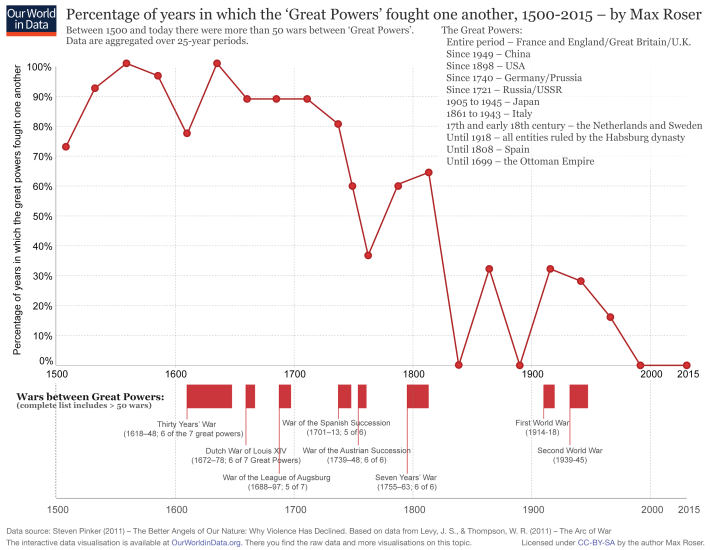
\includegraphics[keepaspectratio, height=\paperheight]{../img/great_powers_wars}};
  \end{tikzpicture}
\end{frame}
% ----------------------------------------------------
\note{Gráfico que muestra la frecuencia de guerras entre grandes potencias a lo largo del tiempo. El patron es claro: desde 1950, las guerras interestatales (especialmente entre grandes potencias) han disminuido dramáticamente. No ha habido guerra entre grandes potencias desde la guerra de Corea (1950-53). Es la paz más larga entre grandes potencias en la historia moderna. Preguntar a los estudiantes: qué ven en el gráfico? ¿Se ha vuelto la guerra obsoleta?}

% ----------------------------------------------------
\begin{frame}[plain]
  \begin{tikzpicture}[remember picture, overlay]
    \node[at = (current page.center), yshift = 0cm] (cover) {%
      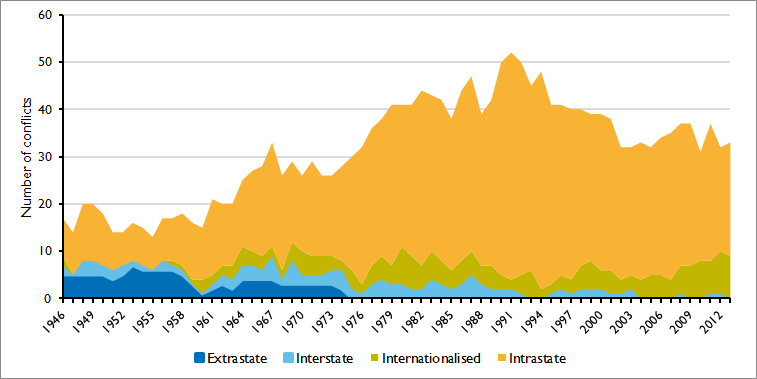
\includegraphics[keepaspectratio, height=\paperheight]{../img/armed_conflicts}};
  \end{tikzpicture}
\end{frame}
% ----------------------------------------------------
\note{Gráfico de conflictos armados (probablemente del UCDP/PRIO). Mostrar que mientras las guerras interestatales han bajado, los conflictos armados en general no han desaparecido. Guerras civiles, conflictos internacionalizados, violencia organizada siguen siendo frecuentes. La guerra interestatal clásica ha declinado, pero la violencia armada no ha desaparecido. Ucrania, Gaza, Sudan, Etiopia, Myanmar...}

% ----------------------------------------------------
\begin{frame}
\frametitle{¿Por qué menos guerras? (Aplicando el marco I-I-I)}
\centering

\begin{itemize}
  \item \textbf{Cambio de intereses:} el territorio ha perdido importancia
  \begin{itemize}
    \item Comercio vs. conquista; nacionalismo encarece la ocupación
  \end{itemize}
  \vspace{8pt}
  \item<2-> \textbf{Costes crecientes:} armas nucleares e interdependencia
  \begin{itemize}
    \item Destrucción mutua asegurada; costes comerciales de la guerra
  \end{itemize}
  \vspace{8pt}
  \item<3-> \textbf{Mejores instituciones:} democracia y organizaciones internacionales
  \begin{itemize}
    \item Paz democrática; verificación (OIEA); mediación (ONU)
  \end{itemize}
\end{itemize}

\end{frame}
% ----------------------------------------------------
\note{Tres factores que explican el declive de la guerra interestatal, conectando con todo lo visto en la sesión. Intereses: en el siglo XIX, la conquista territorial era rentable. Hoy, el comercio internacional permite acceder a recursos sin conquistar. Además, el nacionalismo hace que las poblaciones conquistadas resistan (Irak, Afganistan). Costes: las armas nucleares han hecho que la guerra entre grandes potencias sea potencialmente suicida. La interdependencia económica significa que una guerra destruye cadenas de suministro y mercados. Instituciones: la democracia reduce la probabilidad de guerra entre democracias (paz democrática). Las organizaciones internacionales (OIEA, ONU) mejoran la información y facilitan los compromisos. Pero la guerra no ha desaparecido: Ucrania (2022), Gaza (2023), Sudan (2023). Conectar con la sesión siguiente sobre guerras civiles y nuevas formas de violencia.}


% ====================================================

% ----------------------------------------------------
\begin{frame}
\frametitle{Resumen}
\centering

\begin{itemize}
  \item La guerra es \textbf{costosa} $\rightarrow$ siempre existe un rango de negociación
  \item Pero la negociación puede fallar por:
  \begin{enumerate}
    \item \textbf{Información incompleta} sobre capacidades y determinación
    \item \textbf{Problemas de compromiso} (bienes que dan poder, prevención, preemptividad)
    \item \textbf{Bienes indivisibles} ligados a valores fundamentales
  \end{enumerate}
  \vspace{8pt}
  \item<2-> Señales costosas intentan resolver (I) pero son peligrosas
  \item<3-> La guerra interestatal ha declinado, pero no ha desaparecido
\end{itemize}

\end{frame}
% ----------------------------------------------------
\note{Resumen final de la sesión. Recapitular los tres pilares del tema: el rango de negociación (la guerra siempre destruye valor para ambos bandos), las tres causas de fracaso (información incompleta, problemas de compromiso, bienes indivisibles), y la tendencia histórica de declive de la guerra interestatal. Conectar con la próxima sesión: la semana que viene veremos las guerras civiles, los actores no estatales y el terrorismo. Los conflictos no han desaparecido -- han cambiado de forma.}

% ----------------------------------------------------
\begin{frame}
\frametitle{}
\centering

Preguntas?

\end{frame}
% ----------------------------------------------------
\note{}
